\documentclass{ctexart}

\usepackage{ctex}
\usepackage{tikz}
\usetikzlibrary{calc,positioning,shapes.geometric}
\usepackage{url}
\usepackage{graphicx}
\usepackage{float}
\usepackage{xcolor}
\usepackage{color}
\usepackage{amsmath}
\usepackage{amsthm}
\usepackage{amssymb}
\usepackage{mathrsfs}
\usepackage{caption}
\usepackage{subfigure}
\usepackage{framed}
\usepackage{booktabs}
\usepackage{makecell}
\usepackage{geometry}
\usepackage{wrapfig}
\usepackage{abstract}
\usepackage{algorithmicx}
\usepackage[ruled]{algorithm}
\usepackage{algpseudocode}
\usepackage{setspace}
\usepackage{bm}
\usepackage{cite}
\usepackage{array}
\usepackage{textcomp}
\usepackage{listings}

\definecolor{shadecolor}{rgb}{0.93,0.93,0.93}
\usepackage{geometry}
\geometry{right=2.5cm,left=2.5cm}

\newtheorem{theorem}{定理}

\pagenumbering{arabic}

\begin{document}
\begin{sloppypar}
\title{\vspace{-3cm} \textbf{数值分析项目一作业报告}}
\author{刘陈若\;$3200104872$\\信息与计算科学2001}
\date{}

\maketitle

\section{程序编译和运行说明}
本次项目作业采用Makefile文件对编译进行统一管理。具体地,在Makefile所在目录下输入\verb|make run|
即可完成编译,得到\verb|test.cpp|的可执行文件\verb|test|,对其进行运行即可得到程序结果。

需要说明两点:首先,本项目作业使用eigen3进行线性方程组求解,并使用json file进行参数输入,它们分别以\verb|#include <eigen3/Eigen/...>|和\verb|#include <jsoncpp/json/json.h>|的形式被调用,因此在编译时需要保持相应的文件关系;其次,在使用json file进行参数输入时,部分参数可能需要修改,参数的含义以及具体的修改方式都将在下文中详细给出。

\section{程序运行结果及简要分析}
\subsection{FD.h 设计思路}
在\verb|spline.h|头文件中,一共设计了\verb|Function|,\verb|Circle|和\verb|FD|三个基类,派生出不同的class以满足项目要求。以下将分别展开设计思路叙述。
\subsubsection{class Function}
\verb|Function|类一共设计了\verb|operator()|(括号重载),\verb|diff_x|,\verb|diff_y|和\verb|Laplace|四个虚函数,用于返回给定二元函数的值,其一阶偏导数的值以及-Laplace算子作用后的值。\verb|Function|类主要功能是:存储待求解函数$u$的真实表达式以便输入边界条件并进行误差分析。

\subsubsection{class Circle}

这个类实现了一个圆的基本功能,包括圆心和半径的存储,计算点$P$处的与圆心连线的单位外向量,计算直线与圆的交点(如果存在),以及返回圆心和半径。通过这个类,可以方便地进行圆形几何的计算和处理。其中,函数\verb|get_normal|可以用于计算单位外法方向,函数\verb|get_intersection|可以用于计算直线与圆的交点,函数\verb|get_center|和函数\verb|get_radius|可以用于获取圆心和半径的值。\verb|Circle|类主要功能是存储项目要求中不规则区域的圆。

\subsubsection{class FD}
\verb|FD|类主要功能是实现基于FD method的微分方程数值解的求解。\verb|FD|类一共设计了\verb|solve|,\verb|get_result|和\verb|get_errornorm|三个虚函数,分别用于进行FD算法,返回计算得到的格点处的数值解以及返回误差的1,2以及无穷范数。通过继承这个类,可以创建各种具体的数值解算法,例如针对单位正方形上的偏微分方程和针对单位正方形除去一个圆的偏微分方程。

$\bullet \;$\verb|class FD_regular|:该派生类用于支持单位正方形上的微分方程的Dirichelet,Neumann和mixed三种边界条件求解。\verb|FD_regular(Function &_u, double _h, int _condition)|构造函数,用于接收真实函数值、网格宽度和边界条件等参数。

\verb|solve|函数求解 $AU = F$ 的线性方程组,其中$A$和$F$分别为系数矩阵和右侧向量。我们加入边界作为ghost point,并且按从左到右,从下到上的顺序给格点标序号以便后续计算。该函数在满足不同的边界条件下,使用不同的方法来构造$A$和$F$:当\verb|condition=1|时,表示Dirichlet边界条件。此时,在矩阵A的内部区域中,使用五点差分公式来近似求解二阶偏微分方程。在边界上,将$u$的值作为已知量,构造出系数矩阵$A$和右侧向量$F$;当\verb|condition=2|时,表示Neumann边界条件。此时,在矩阵$A$的内部区域中,仍然使用五点差分公式来近似求解二阶偏微分方程。但是在边界上,我们根据FD formula得到的二阶精度的导数来作为导数值(左右边界为关于$x$的偏导数,上下边界为关于$y$的偏导数)的估计。需要注意的是,左右两边以及上下两边对应的系数是相反的;当\verb|condition=3|时,表示mixed边界条件,在本程序中假设左右两边为Neumann,上下两边为Dirichlet,此时将以上两种方法结合使用即可构建方程组。

\verb|get_result|和\verb|get_errornorm|的作用已在前文叙述,此处不再赘述。

$\bullet \;$\verb|class FD_irregular|:该派生类用于支持单位正方形内部去掉一个圆的区域上的微分方程的Dirichelet,Neumann和mixed三种边界条件求解。\verb|FD_irregular|构造函数,用于接收真实函数值,网格宽度,边界条件和圆的信息等参数。

\verb|Label|函数返回一个vector $L$,其每个元素代表一个需要求解的点以及其类型。具体来说,对于一个二维区域,其第i个元素为$\left\{x_i,y_i,type_i\right\}$,其中$(x_i,y_i)$是对应序号i的点的坐标,$type_i$为点的类型:$type_i=1$为区域内格点,$type_i=2$为区域外ghost point(四周存在一个区域内格点,且不在边界上的点),$type_i=3$为正方形边界点,$type_i=4$为恰好落在圆上的格点。函数中的实现逻辑是遍历整个区域内的点,根据其距离区域内挖去的圆的距离以及是否在边界上来确定其类型,并将其加入到返回的vector中。同时,再判断全体格点是否为ghost point。最后返回所有点的信息。

\verb|Find_Label|函数用于查找给定坐标在vector $L$中的位置和类型。如果该点不在$L$中,返回 $\left\{-1,-1\right\}$。

\verb|solve|函数求解 $AU = F$ 的线性方程组,其中$A$和$F$分别为系数矩阵和右侧向量。我们对vector $L$中的元素进行便利,在不同的边界条件下,使用不同的方法来构造$A$和$F$:当\verb|condition=1|时,表示Dirichlet边界条件。此时,在矩阵A的内部区域中,使用五点差分公式来近似求解二阶偏微分方程。在边界上,将$u$的值作为已知量,构造出系数矩阵$A$和右侧向量$F$。比较不同的是$type_i=2$的情况,此时我们从该点按上下右左的顺序依次搜索,找到与其相邻的(第一个)内点以及对应的圆与网格的交点,从而用线性插值的方式得到一个方程;当\verb|condition=2|时,表示Neumann边界条件。此时,在矩阵$A$的内部区域中,仍然使用五点差分公式来近似求解二阶偏微分方程,在正方形边界上的做法也和\verb|FD_regular|相同。但是在圆形边界上的情况会有所不同,此时将圆和网格交点对应的$type_i=2$的点处通过上下左右一次搜索,用周围的四个点对方向导数进行二阶精度表示,以近似交点处的方向导数;当\verb|condition=3|时,表示mixed边界条件,在本程序中假设正方形边界为Neumann,圆形边界为Dirichlet,此时$type_i$的各种取值对应的情况都可以用上文中相应方法得到解决。

\verb|get_result|和\verb|get_errornorm|的作用已在前文叙述,此处不再赘述。

\textbf{注}:1.关于Neumann编制条件以及非规则区域的搜索方法较为繁琐(但是思路是很清晰的),本人文字表达能力有限,如果有没有表达清楚的地方烦请在\verb|FD.h|中找到相应的代码,我已尽量作出完整的注释;2.Neumann边值的情况由于得到的解不适定,需要增加额外非导数的条件,本程序用序号为1的点对应的真实值作为补充条件。

\subsection{程序测试指南及结果展示}
本节中,我将说明如何对程序\verb|test.cpp|进行测试,并根据题目要求完成对函数进行求解和误差分析,以及对结果给出可视化的展示(图像均由Python绘制)。

\subsubsection{test.json 参数说明}
所有的任务都可以通过调整\verb|test.json|中的参数得到解决。因此本节首先给出\verb|test.json|中各参数的含义说明。

$\bullet \;$ \verb|n|:单位正方形格点等分数(沿$x$以及$y$方向)。根据题目要求$n=8,16,32,64$,一般无需修改。

$\bullet \;$ \verb|function_label|:函数标号。根据题目要求,设计了三个函数进行求解,序号1代表$u = e^{y+\sin x}$,序号2代表$u = e^{-xy}$,序号3代表$u = \sin(xy)$,可根据需求自行修改。

$\bullet \;$ \verb|circle|:区域中需要挖掉的圆的信息。需要输入三个浮点数,第一个代表圆心的$x$坐标,第二个代表圆心的$y$坐标,第三个代表圆的半径。如果区域$\omega$为单位正方形,则将半径设置为0即可。

$\bullet \;$ \verb|boundary_condition|:输入1,2,或3,代表边界条件。1表示Dirichlet,2表示Neumann, 3表示mixed。

\subsubsection{test.cpp 输出说明}
针对不同的参数运行\verb|test.cpp|,得到的结果(包括误差范数,在固定点的误差,在格点处的值等)全部输出至文件\verb|test_results.txt|中,根据需要进行选择即可。

\subsubsection{数值求解结果展示}
在求解方程之后,通过\verb|get_result|可以得到每一个格点处的$u$的数值解并将其输出至\verb|test_results.txt|中,据此可以绘制图像进行清晰地展示。由于对三个函数对应的所有$n$和边界条件进行绘图将会得到几十幅图像,一一列举并不现实,加之本人并没有足够的Python水平绘制出挖掉一个圆的立体图,此处仅选取部分数值结果图像进行展示。

具体来说,首先对$n=8,16,32,64$,绘制正方形区域函数$u = e^{y+\sin x}$对应Dirichlet边值条件的求解结果的图像如下所示。
\begin{figure}[H]
  \begin{minipage}[t]{0.5\linewidth}
    \centering
    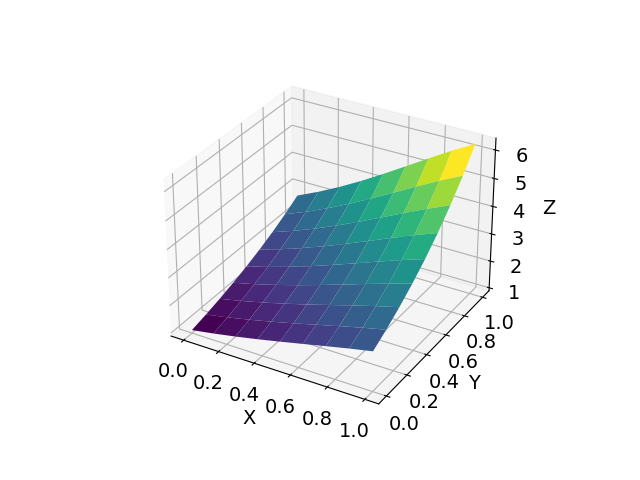
\includegraphics[scale = 0.5]{f1_D_8.png}
    \caption{$n = 8$}
  \end{minipage}
  \begin{minipage}[t]{0.5\linewidth}
    \centering
    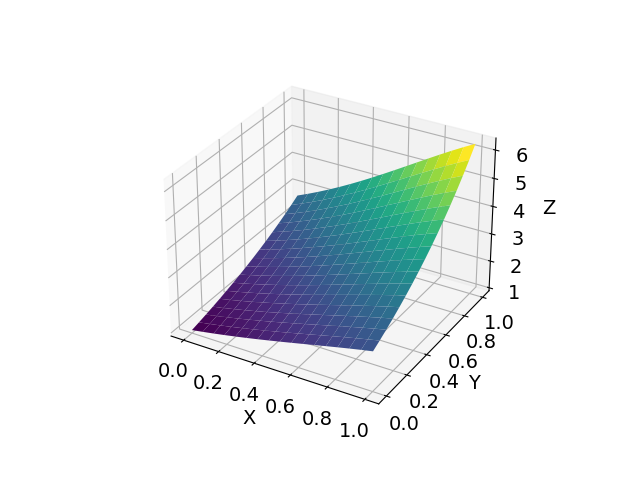
\includegraphics[scale = 0.5]{f1_D_16.png}
    \caption{$n = 16$}
  \end{minipage}
  \label{fig2}
\end{figure}

\begin{figure}[H]
  \begin{minipage}[t]{0.5\linewidth}
    \centering
    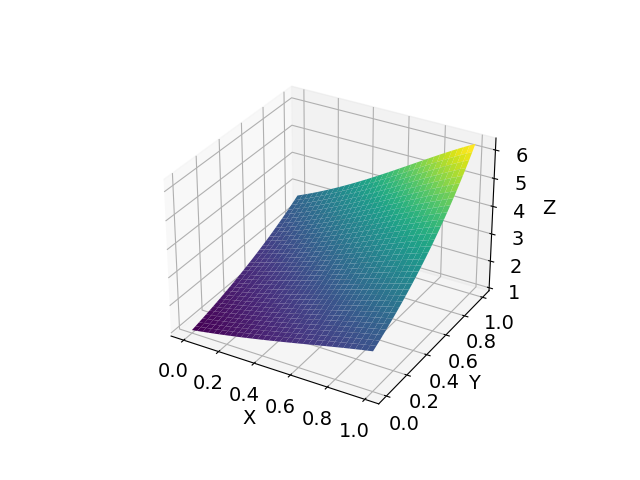
\includegraphics[scale = 0.5]{f1_D_32.png}
    \caption{$n = 32$}
  \end{minipage}
  \begin{minipage}[t]{0.5\linewidth}
    \centering
    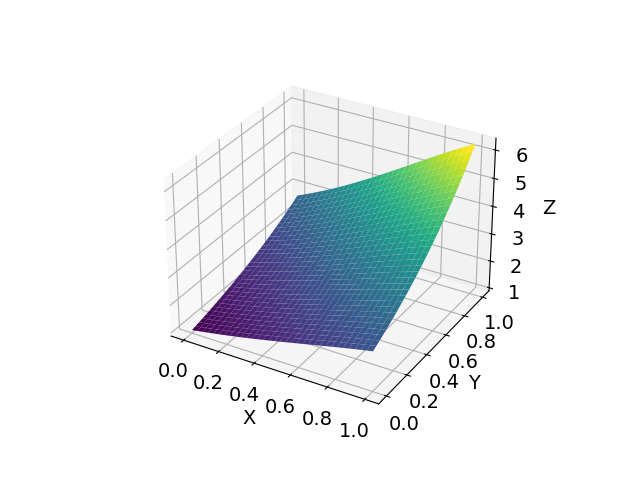
\includegraphics[scale = 0.5]{f1_D_64.png}
    \caption{$n = 64$}
  \end{minipage}
  \label{fig2}
\end{figure}

其次,对$n=8,16,32,64$,绘制正方形区域函数$u = e^{-xy}$对应Neumann边值条件的求解结果的图像如下所示。
\begin{figure}[H]
  \begin{minipage}[t]{0.5\linewidth}
    \centering
    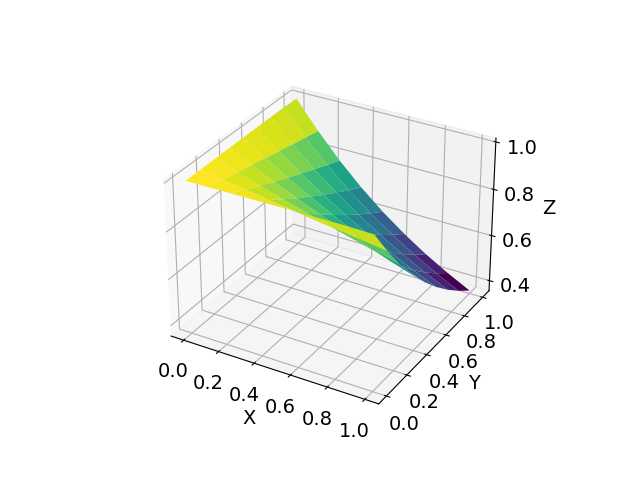
\includegraphics[scale = 0.5]{f2_N_8.png}
    \caption{$n = 8$}
  \end{minipage}
  \begin{minipage}[t]{0.5\linewidth}
    \centering
    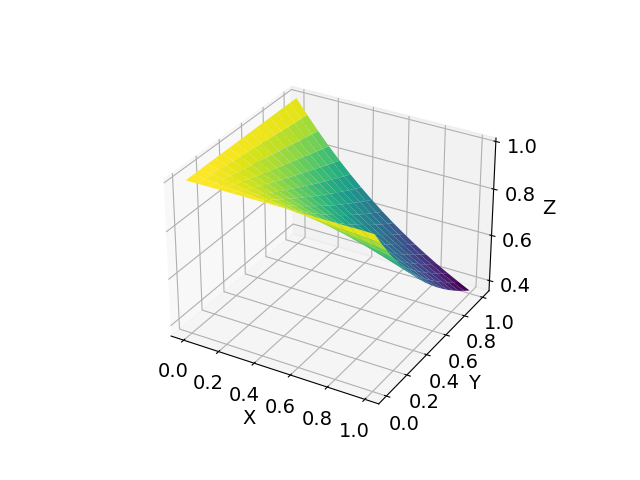
\includegraphics[scale = 0.5]{f2_N_16.png}
    \caption{$n = 16$}
  \end{minipage}
  \label{fig2}
\end{figure}

\begin{figure}[H]
  \begin{minipage}[t]{0.5\linewidth}
    \centering
    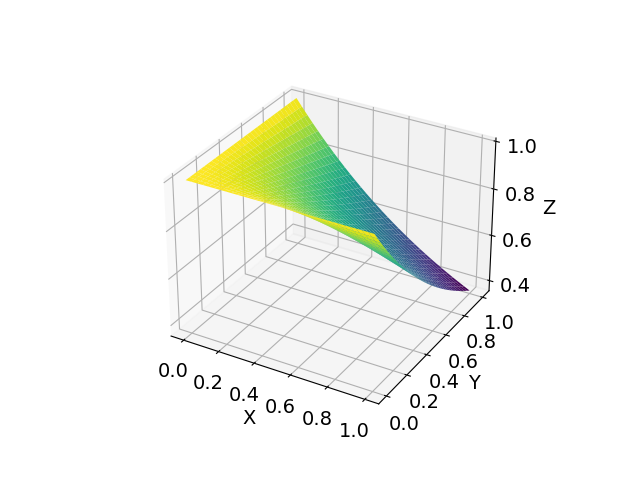
\includegraphics[scale = 0.5]{f2_N_32.png}
    \caption{$n = 32$}
  \end{minipage}
  \begin{minipage}[t]{0.5\linewidth}
    \centering
    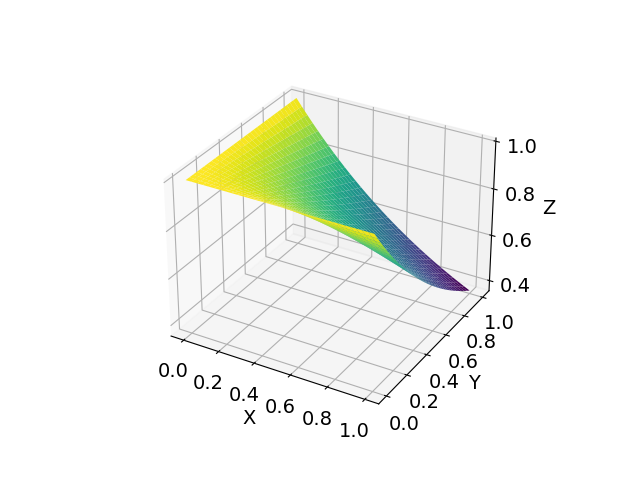
\includegraphics[scale = 0.5]{f2_N_64.png}
    \caption{$n = 64$}
  \end{minipage}
  \label{fig2}
\end{figure}

最后,对$n=8,16,32,64$,绘制正方形区域函数$u = \sin(xy)$对应Mixed边值条件的求解结果的图像如下所示。
\begin{figure}[H]
  \begin{minipage}[t]{0.5\linewidth}
    \centering
    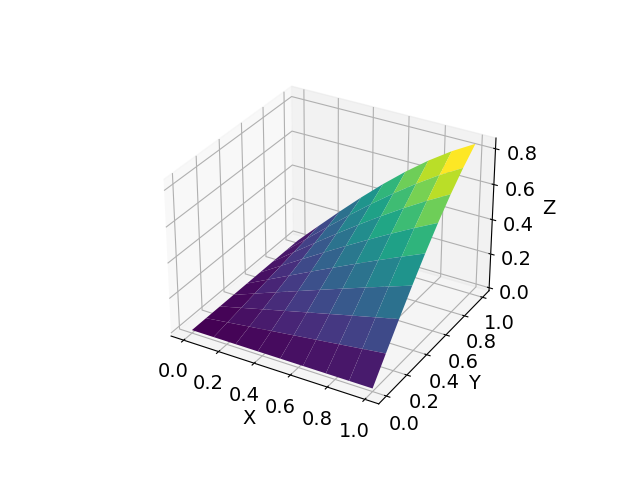
\includegraphics[scale = 0.5]{f3_M_8.png}
    \caption{$n = 8$}
  \end{minipage}
  \begin{minipage}[t]{0.5\linewidth}
    \centering
    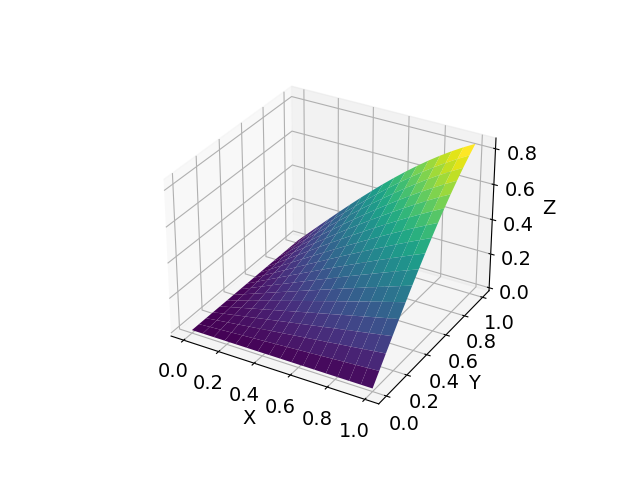
\includegraphics[scale = 0.5]{f3_M_16.png}
    \caption{$n = 16$}
  \end{minipage}
  \label{fig2}
\end{figure}

\begin{figure}[H]
  \begin{minipage}[t]{0.5\linewidth}
    \centering
    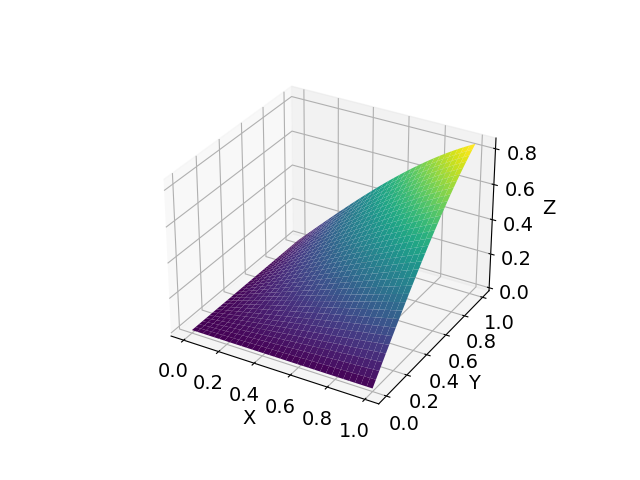
\includegraphics[scale = 0.5]{f3_M_32.png}
    \caption{$n = 32$}
  \end{minipage}
  \begin{minipage}[t]{0.5\linewidth}
    \centering
    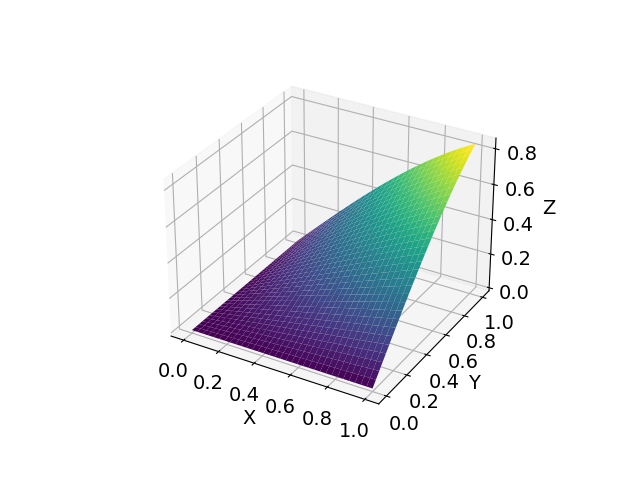
\includegraphics[scale = 0.5]{f3_M_64.png}
    \caption{$n = 64$}
  \end{minipage}
  \label{fig2}
\end{figure}

从图像中我们可以很好地看出各个函数在单位正方形内的变化趋势,这从直观上验证了\verb|FD.h|中关于FD method的算法的有效性,也展示了FD method能够较好的对原函数进行估计。对于不规则区域,接下来的误差分析中也可以从中反映算法的正确性和有效性。

\subsubsection{固定点收敛速率分析}
根据题目要求,在程序运行时,我们记录下求解结果与真实解在四个点$(0.125,0.125)$,$(0.125,0.875)$,$(0.875,0.125)$和$(0.875,0.875)$的绝对误差输出至\verb|test_results.txt|中。

为了对收敛速率进行分析,我们需要对获得的绝对误差进行进一步处理。首先,修改\verb|test.json|中\verb|n|为\verb|[8,16,32,64,128]|,增加网格数以便观察趋势;其次,绘制绝对误差序列前一项与后一项的比值,以便观察$n$翻倍之后绝对误差缩减的比例。

基于此,我们首先对规则区域进行收敛阶分析。对于三个函数,我们分别记录每个函数对应的三种边界条件的绝对误差序列的比值(取$\log 2$)。由于有四个点,因此我们取四个点计算得到的平均值。据此绘制图像如图所示。
\begin{figure}[H]
\centering
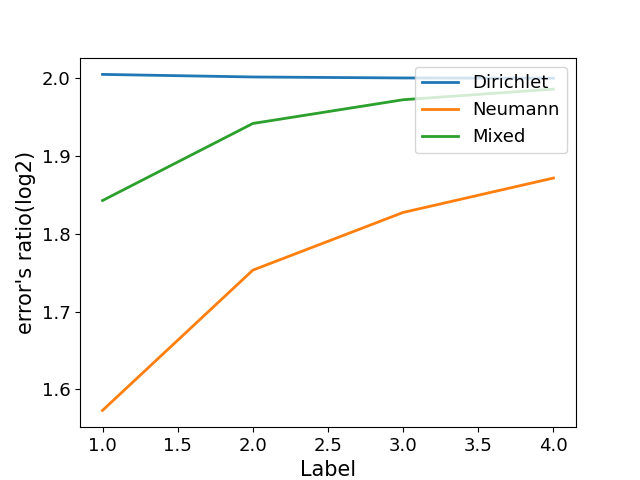
\includegraphics[scale = 0.5]{f1_PE.png}
\caption{规则区域$u=e^{y+\sin x}$误差比值($\log 2$)}
\label{fig7}
\end{figure}

\begin{figure}[H]
  \begin{minipage}[t]{0.5\linewidth}
    \centering
    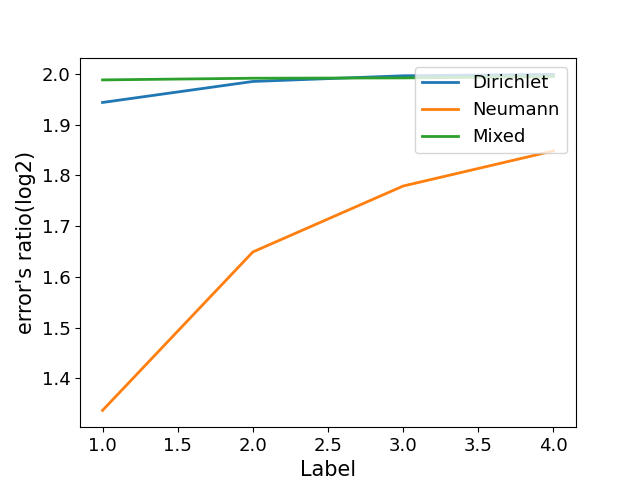
\includegraphics[scale = 0.5]{f2_PE.png}
    \caption{规则区域$u=e^{-xy}$误差比值($\log 2$)}
  \end{minipage}
  \begin{minipage}[t]{0.5\linewidth}
    \centering
    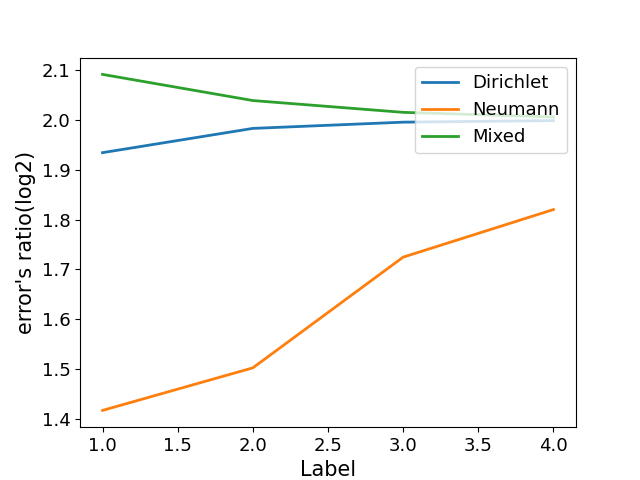
\includegraphics[scale = 0.5]{f3_PE.png}
    \caption{规则区域$u=\sin(xy)$误差比值($\log 2$)}
  \end{minipage}
  \label{fig2}
\end{figure}
从图中可以较直观的看出,\textbf{三种边界条件的收敛速度关于$h$都是2阶的}。具体来说,相较之下Dirichlet和Mixed边值条件的收敛比值较为接近2,且较为稳定;而Neumann边值条件的收敛阶相对较不稳定,但逐渐趋于2。另一方面,根据\verb|test_results.txt|的输出,Dirichlet和Mixed边值条件的误差从量级上也小于Neumann边值条件的误差,这应该是因为纯Neumann的边值问题是不适定的,而本程序仅仅对其增加了一个新的条件,这只能确保该PDE有唯一解,但条件仍较弱,因此得到的数值解的误差较大。

其次,我们对不规则区域进行收敛阶分析。不妨设挖去的圆心在$(0.5,0.5)$,半径为0.25.同样地,对于三个函数,我们分别记录每个函数对应的三种边界条件的绝对误差序列的比值如下图所示。
\begin{figure}[H]
\centering
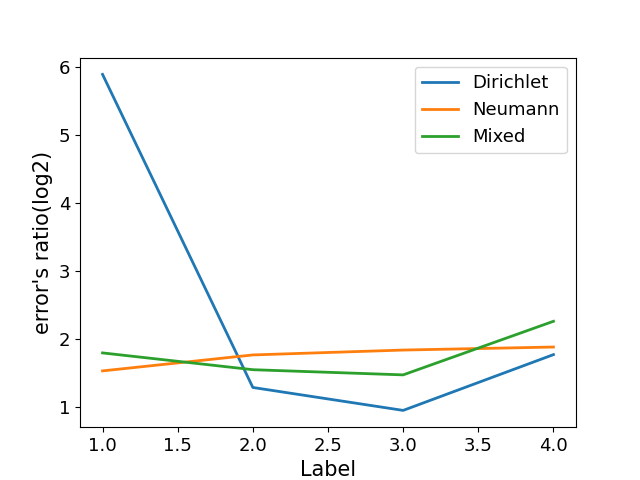
\includegraphics[scale = 0.5]{f1_IPE.png}
\caption{不规则区域$u=e^{y+\sin x}$误差比值($\log 2$)}
\label{fig7}
\end{figure}

\begin{figure}[H]
  \begin{minipage}[t]{0.5\linewidth}
    \centering
    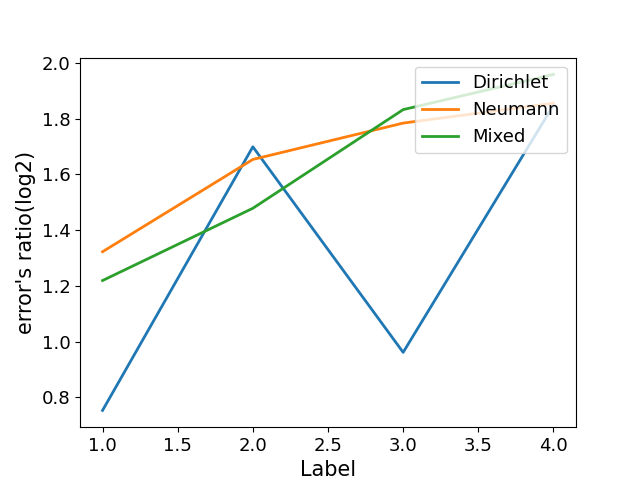
\includegraphics[scale = 0.5]{f2_IPE.png}
    \caption{不规则区域$u=e^{-xy}$误差比值($\log 2$)}
  \end{minipage}
  \begin{minipage}[t]{0.5\linewidth}
    \centering
    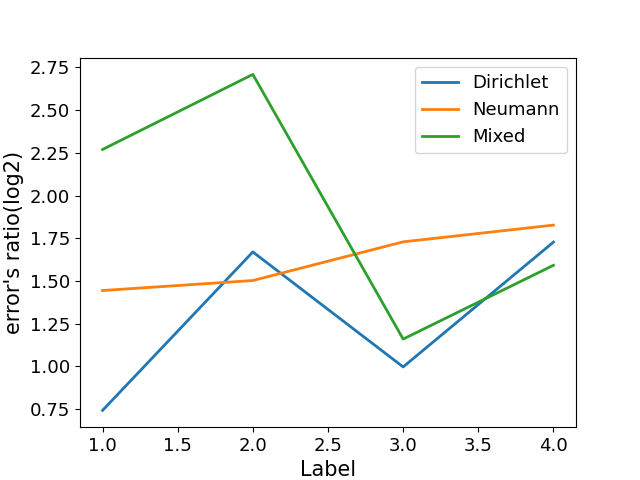
\includegraphics[scale = 0.5]{f3_IPE.png}
    \caption{不规则区域$u=\sin(xy)$误差比值($\log 2$)}
  \end{minipage}
  \label{fig2}
\end{figure}
从总体趋势来看,\textbf{三种边界条件的收敛速度关于$h$依然是2阶的}。区别在于不规则区域Dirichlet和Mixed边值条件的不稳定性相比规则区域变大了。观察\verb|test_results.txt|的输出发现,这是因为此时某个别点的收敛速率严重偏离2阶,而其他点依旧是2阶收敛的。这可能是因为对于ghost point,它的四周可能存在两个或者更多内点,但我们在ghost point只能设置一个边值条件,因此会使得得到的解具有较大的误差。

\subsection{误差范数及其收敛分析}
根据题目要求,\verb|test_results.txt|中还输出了不同函数、边值条件和$n$对应的误差的1、2和无穷范数,其定义为
\begin{equation}
\begin{aligned}
    &\Vert g \Vert_1 = h^2 \sum_i|g_i|, \\
    &\Vert g \Vert_2 = \left(h^2 \sum_i|g_i|^2\right)^{\frac{1}{2}}, \\
    &\Vert g \Vert_{\infty} = \max_i|g_i|.
\end{aligned}
\end{equation}

关于其绝对的值都可以在文本文档中详细查看,可以看出不论何种情况,误差的各范数都是很小的数值(小于$10^{-3}$),这也从侧面印证了算法的正确性。

同样的,我们更加关注的是误差范数的收敛分析。当每个元素时二阶收敛时,根据类似\textbf{Exercise 7.14}的简单运算(注意此时$N=\Theta(\frac{1}{h^2})$),我们可以得到
\begin{equation}
\begin{aligned}
    &\Vert g \Vert_1 = h^2O(1) = O(h^2), \\
    &\Vert g \Vert_2 = h[O(h^2)]^{\frac{1}{2}} = O(h^2), \\
    &\Vert g \Vert_{\infty} = O(h^2),
\end{aligned}
\end{equation}
这也是我们所需要验证的。
首先,修改\verb|test.json|中\verb|n|为\verb|[8,16,32,64,128]|,增加网格数以便观察趋势;其次,绘制误差范数序列前一项与后一项的比值,以便观察$n$翻倍之后绝对误差缩减的比例。

基于此,我们首先对规则区域进行收敛阶分析。对于三个函数,我们分别记录每个函数对应的三种误差范数的比值(取$\log 2$),据此绘制图像如图所示。(根据上一节分析,各点的收敛阶均为2,因此为了避免图像过多,不失一般性,此处仅展示Dirichlet边值条件的结果)。
\begin{figure}[H]
\centering
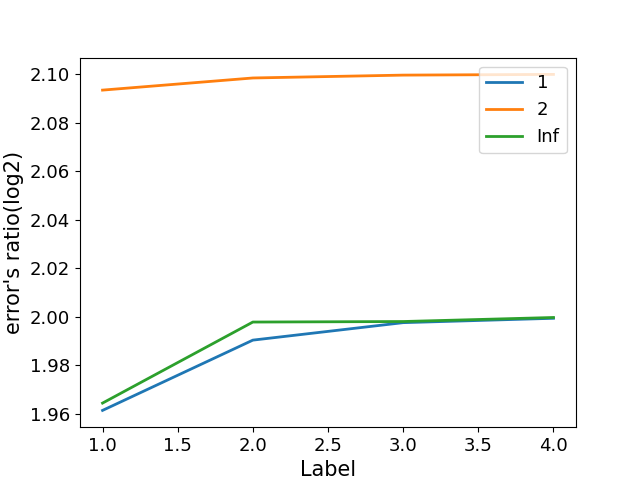
\includegraphics[scale = 0.5]{f1_NE.png}
\caption{规则区域$u=e^{y+\sin x}$误差范数比值($\log 2$)}
\label{fig7}
\end{figure}

\begin{figure}[H]
  \begin{minipage}[t]{0.5\linewidth}
    \centering
    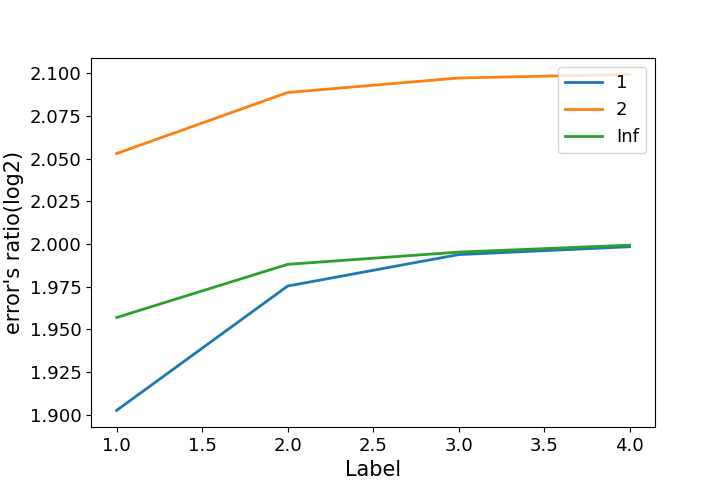
\includegraphics[scale = 0.5]{f2_NE.png}
    \caption{规则区域$u=e^{-xy}$误差范数比值($\log 2$)}
  \end{minipage}
  \begin{minipage}[t]{0.5\linewidth}
    \centering
    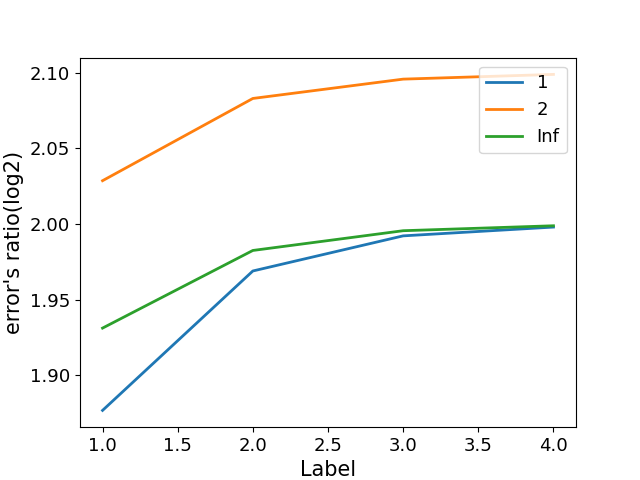
\includegraphics[scale = 0.5]{f3_NE.png}
    \caption{规则区域$u=\sin(xy)$误差范数比值($\log 2$)}
  \end{minipage}
  \label{fig2}
\end{figure}
显然,\textbf{规则区域三种范数的收敛阶都稳定趋向于2附近},这在计算机层面验证了前文所述的收敛速率。(不过三个函数的二范数都趋向于2.1左右,这个现象我并没有想明白是为什么)。

其次,我们对不规则区域进行收敛阶分析。不妨设挖去的圆心在$(0.5,0.5)$,半径为0.25.同样地,对于三个函数,我们分别记录每个函数对应的三种误差范数的比值(取$\log 2$),据此绘制图像如图所示。(根据上一节分析,各点的收敛阶均为2,因此为了避免图像过多,不失一般性,此处仅展示Neumann边值条件的结果)。
\begin{figure}[H]
\centering
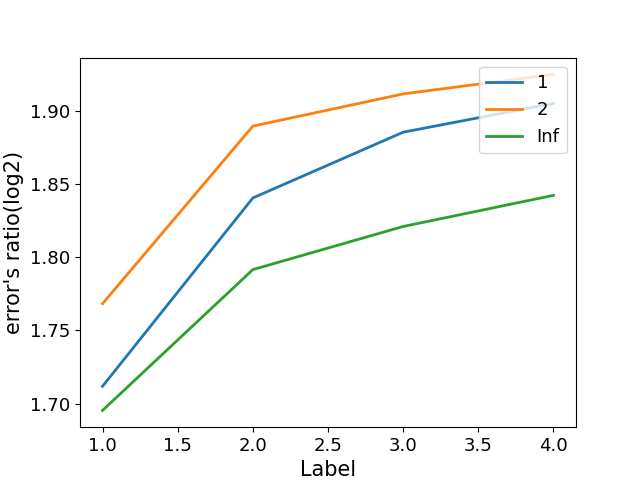
\includegraphics[scale = 0.5]{f1_INE.png}
\caption{不规则区域$u=e^{y+\sin x}$误差比值($\log 2$)}
\label{fig7}
\end{figure}

\begin{figure}[H]
  \begin{minipage}[t]{0.5\linewidth}
    \centering
    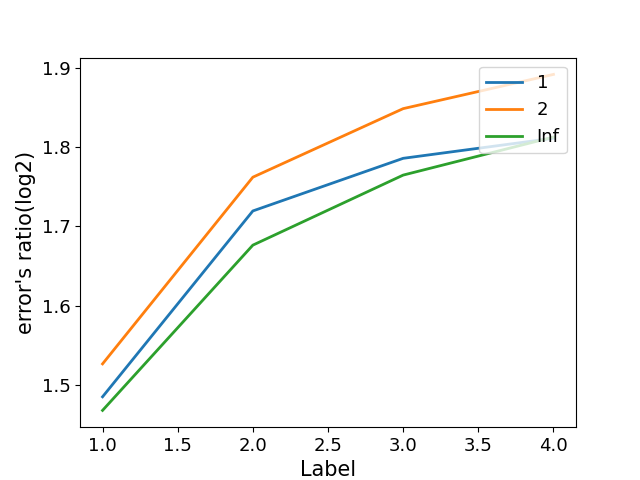
\includegraphics[scale = 0.5]{f2_INE.png}
    \caption{不规则区域$u=e^{-xy}$误差比值($\log 2$)}
  \end{minipage}
  \begin{minipage}[t]{0.5\linewidth}
    \centering
    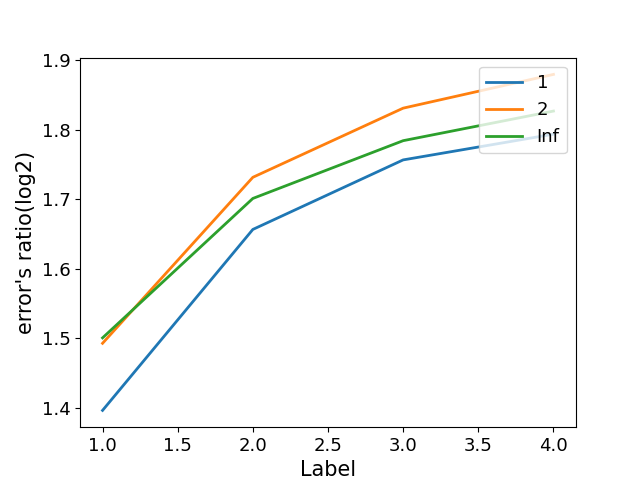
\includegraphics[scale = 0.5]{f3_INE.png}
    \caption{不规则区域$u=\sin(xy)$误差比值($\log 2$)}
  \end{minipage}
  \label{fig2}
\end{figure}
不难看出,随着网格的加细,\textbf{不规则区域三种范数的收敛阶也都稳定趋向于2附近},这在计算机层面验证了前文所述的收敛速率。
\end{sloppypar}
\end{document}
